\section{Results: ownership, income protection and financing are different margins}
\subsection{What changes when the counterfactual is strengthened?}
Table~\ref{tab:comparison} summarises the new 50-year medium-automation comparison. The values describe a synthetic scenario. Equal starting conditions permit controlled comparison, but the behavioural equations and policy functions are not empirically identified.

\begin{table}[htbp]\centering\small
\caption{Medium automation, model year 50: strengthened policy comparisons}\label{tab:comparison}
\begin{tabular}{@{}lrrrrr@{}}
\toprule
Policy & $Y_{50}$ & MVI/GDP & Tax/GDP & Participant/GDP & Book Gini \\
\midrule
B0 & 6.48 & 7.07 & 25.01 & 0.00 & 0.768 \\
B2 & 6.48 & 19.03 & 37.04 & 0.00 & 0.754 \\
B5 & 6.48 & 10.57 & 28.53 & 17.14 & 0.583 \\
B6 & 6.48 & 10.16 & 27.13 & 17.14 & 0.584 \\
B7 & 6.48 & 5.96 & 23.91 & 17.14 & 0.560 \\
B10 & 6.48 & 16.98 & 34.98 & 0.00 & 0.749 \\
B11 & 6.48 & 10.57 & 28.53 & 17.14 & 0.745 \\
B12 & 6.48 & 10.16 & 27.13 & 17.14 & 0.749 \\
B13 & 6.48 & 1.91 & 18.75 & 17.14 & 0.595 \\
\bottomrule
\end{tabular}

\par\smallskip\footnotesize Flow columns are percentages of GDP. B0: targeted transfers; B2: universal transfers; B5: user equity; B6: user equity plus monetary levy; B7: equal equity; B10: capital-focused tax; B11/B12: matched levies for B5/B6; B13: targeted hybrid. Tax/GDP excludes earmarked participant pass-through levies, which equal 17.14\% of GDP in B11/B12. Book Gini excludes capitalised future fiscal claims.
\end{table}

Relative to B2, adding user equity in B5 reduces MVI by 8.46 percentage points of GDP, from 19.03\% to 10.57\%. Adding the monetary holding-levy architecture in B6 contributes a further 0.41 percentage points, bringing MVI to 10.16\%. Approximately 95\% of the combined transfer reduction along this sequential comparison precedes the special levy. This is an order-dependent ablation, not a structural attribution or a Shapley decomposition. B5's book-wealth Gini of 0.583 is marginally lower than B6's 0.584; the monetary instrument is not unambiguously more equalising.

The stronger tax comparator B10 reduces MVI to 16.98\% and conventional tax/GDP to 34.98\%, compared with 19.03\% and 37.04\% in B2. Thus adapting tax incidence helps even without equity grants. The experiment does not search the space of optimal nonlinear taxes, capital-income smoothing or behavioural responses. It supports a comparison against this explicit schedule, not a conclusion that usownership dominates the best possible fiscal system.

Targeting is at least as consequential. B0 requires MVI of 7.07\% of GDP, below the 10.16\% universal hybrid. Combining targeted protection with usownership and the levy in B13 lowers it to 1.91\%, with residual conventional taxation of 18.75\%. Universal and targeted schemes share a reference floor but not the same coverage, information requirements or political contract. Predicted-gap targeting remains imperfect in realised outcomes. The result is therefore a strong reason to separate protection policy from ownership policy, not a proof that means testing is always preferable.

\begin{figure}[htbp]\centering
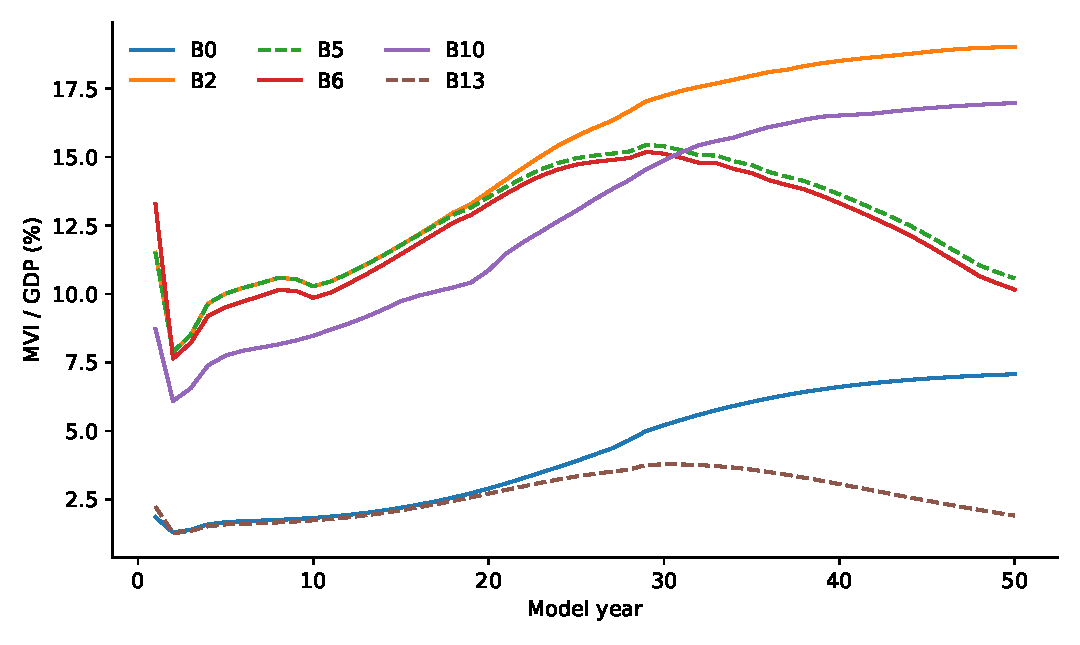
\includegraphics[width=.90\linewidth]{figures/comparative_transfer.pdf}
\caption{MVI paths under strengthened counterfactuals. Targeting and ownership each matter; the holding levy is a smaller incremental change in this scenario.}
\end{figure}

\subsection{The matched levy removes the claim of automatic cash-flow superiority}
B11 reproduces B5 and B12 reproduces B6 in household cash income, consumption, MVI, monetary balances, prices and output. Across three automation paths and eight recorded macro metrics for each matched pair, the maximum discrepancy is zero at the exported numerical precision. This is an implementation check of Proposition~\ref{prop:equivalence}, not an independent empirical finding.

The register reallocates 17.14\% of GDP in participant cash income at year 50 under either legal form in the medium path. In B6 this is user dividends; in B12 it is an earmarked levy rebate. Ordinary tax/GDP is 27.13\% in each. Including the gross pass-through, B12 records total taxes of 44.27\% of GDP and an equal additional rebate flow. That larger gross tax number does \emph{not} establish a larger net resource burden or lower efficiency. It is the cash-flow analogue of the in-kind equity redistribution.

Legal book ownership does differ: user equity is 29.67\% in B6 and zero in B12. Their book-wealth Ginis are 0.584 and 0.749. Because future tax and rebate claims are not included in that measure, it cannot adjudicate their economic net wealth or welfare. An equal-payoff valuation would capitalise both the legacy owners' levy liability and the participants' rebate asset. The genuine remaining research questions concern enforceability, control, transferability, risk and participation responses. They are not solved by the wealth-accounting label.

\begin{figure}[htbp]\centering
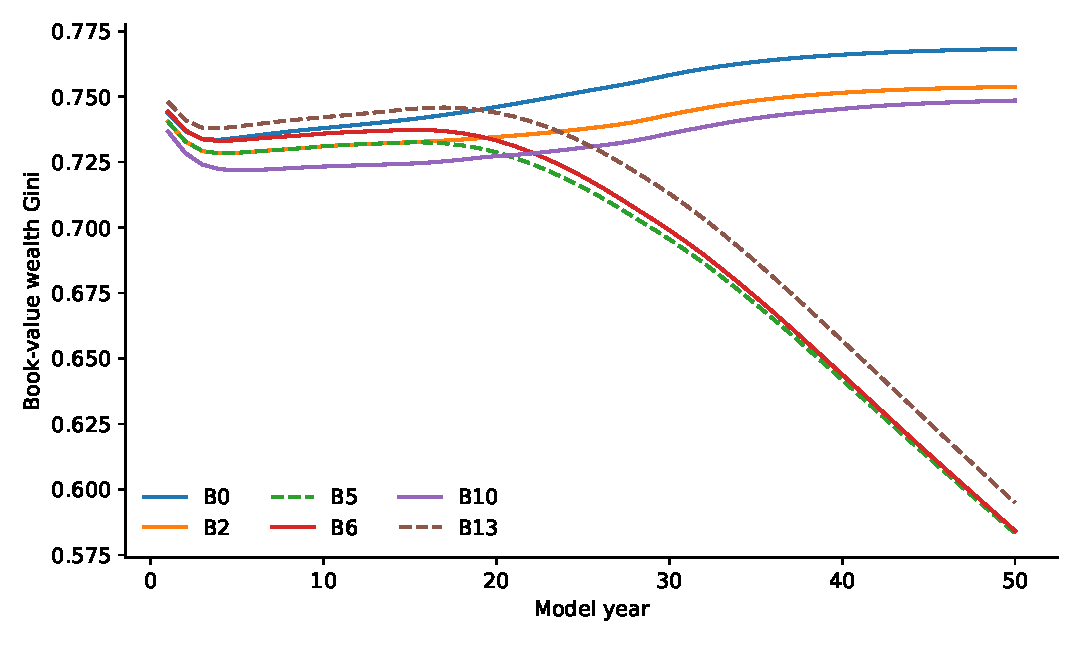
\includegraphics[width=.90\linewidth]{figures/comparative_ownership.pdf}
\caption{Legal book-wealth concentration. These series exclude capitalised fiscal claims and must not be read as welfare rankings over matched income streams.}
\end{figure}

\subsection{The financing limit remains binding}
The central B6 hybrid uses conventional taxes of 27.13\% of GDP at year 50. Fiscal issuance before the holding levy is 4.60\% of GDP: 1.31 percentage points correspond to the explicit levy and 3.29 to net monetary financing. Near-target inflation, peaking around 2.13\% over the 50-year path, is conditional on the residual-tax instrument and the price closure.

Fixed-tax monetary financing performs very differently. In the original medium path, B3 reaches roughly 40.3\% peak inflation; adding demurrage in B4 raises that peak to roughly 45.1\%. The induced reduction in desired balances can outweigh part of the mechanical cancellation effect. These are model-specific counterexamples, not predictions that negative interest is always inflationary. The central no-conventional-tax case fails numerically before substantial ownership diffusion. Extreme rates near the numerical stop are diagnostics, not quantitative hyperinflation forecasts.

A narrower no-tax case retains the original proposal's 7\% public-purchases block, sets the income reference to 15\% and initial money/GDP to one. It survives 50 years and eventually has no top-up, but peak inflation is about 7.03\%, outside the strict 5\% band. It does not maintain the central public-service commitment or the 2\% target. This favourable counterexample is retained because the relevant object is a feasible financing region, not an unconditional impossibility claim. Higher money demand is an assumption, not a policy instrument that can simply be ordered into existence.

\begin{figure}[htbp]\centering
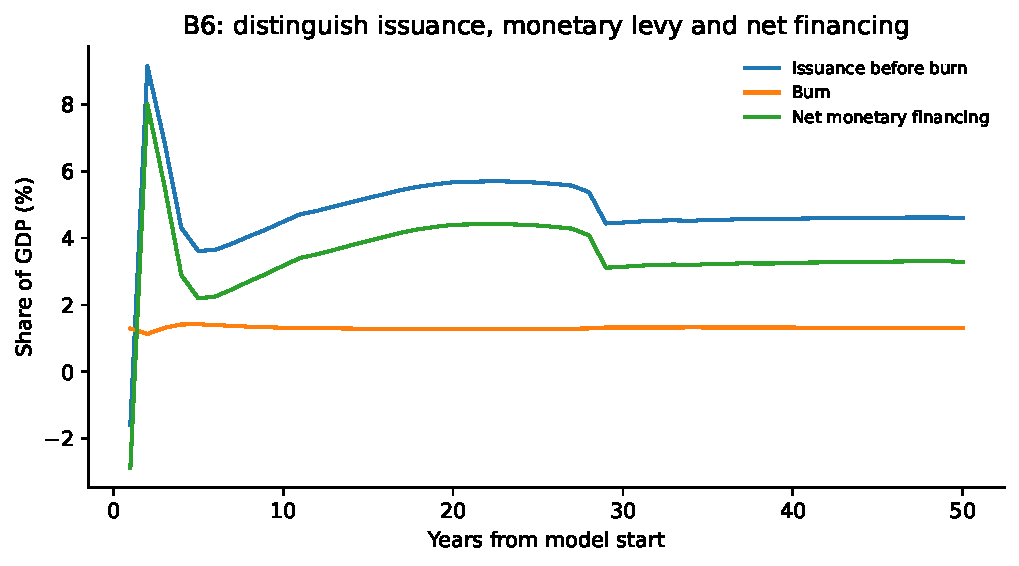
\includegraphics[width=.90\linewidth]{figures/monetary_flows.pdf}
\caption{Money financing in the medium hybrid. Issuance before the holding levy must not be added to that levy as though both were independent free resources.}
\end{figure}

\subsection{Coverage and the speed of the ownership bridge}
The original medium hybrid's MVI/GDP peaks near 15.19\% in year 29, then falls to 10.16\% in year 50. It does not disappear within that window. Only six of the 128 original hybrid parameter configurations meet the specified five-year sunset criterion; the corresponding counts are four for B5 and zero for B2. These frequencies describe the chosen parameter box, not probabilities of real-world success. A prosperity-indexed floor is harder to replace than a fixed-real floor because growing output also raises the income objective.

The participant selection mechanism is crucial. Excluding the lowest-initial-wage 20\% from equity grants leaves aggregate user ownership unchanged but raises MVI to about 19.15\% of GDP at year 50. Large aggregate capital claims do not help a person who does not receive them. The equal-grant B7 comparator lowers MVI to 5.96\% and the book Gini to 0.560, outperforming contribution weighting on these distributional metrics. Since contribution-related effort gains are not estimated, there is no basis for treating this as an inferior policy. It is a transparent trade-off between the participation rationale and broad coverage, not an instruction to replace the user's firm-specific design with a pooled fund.

Consumption-only allocation, score capture and early sales weaken the ownership result in the inherited robustness runs. Immediate permitted liquidation leaves user equity around 7.72\% and a book Gini near 0.753; ten-year vesting with a retained core moderates that channel. However, restrictions cost liquidity and diversification. People facing disability, care obligations or poor digital access must not be required to supply behavioural data merely to obtain subsistence support. The MVI floor and participant equity remain separate entitlements.

\subsection{Output and investment are not free gains}
Several medium-automation cases reach exactly the same year-50 real output, 6.481 times the initial index. The resource ceiling binds. This is not evidence that equity diffusion is costless, nor that any policy generates a growth dividend. In the original unconstrained-resource sensitivity, output at year 50 is about 6.862 with no dilution-investment penalty, 6.738 with the central penalty and 6.227 with a higher penalty. Their differences are consequences of assumed investment responses, not empirical elasticity estimates.

The additional 72 robustness paths compare the strongest practical benchmarks under twelve common parameter settings. They retain adverse cases, rather than selecting only a favourable equity path. The full machine-readable results include coverage gaps, residual taxation and the log-consumption diagnostic as well as wealth. No welfare-superiority claim is based on a single Gini or on nominal GDP growth. The unresolved investment, governance and participation responses are precisely the parameters needed for an empirical test of the institutional advantage in \eqref{eq:wedge}.
